\chapter{Gas Electron Multiplier Detectors}
\label{chap:II-1-gem}

  In 1968, G. Charpak revolutionized the field of tracking detectors by introducing the Multiwire Proportional Chamber (MWPC). MWPCs were more reliable than the existing single-wire gas counters providing a higher sub-mm resolution and rate capabitilies up to fluxes of several MHz cm$^{-2}$. Developments of manufacturing technics and high-density electronics led to a new generation of detectors fulfilling the needs of high-energy physics experimentation. However, their use in high-luminosity experiments revealed some intrensic weaknesses: the mechanical design of the chamber limits the spacial resolution; long ion drift times affect the efficiency of the detector at high fluxes; solid deposits aglomerate on the wires due to aging and induce sparks in the chamber. \\

  Twenty years later, Micro-Strip Gas Counters (MSGCs) were developped using photolithographic processes to engrave anode and cathode strips on an insulating support. Both the position resolution and the rate capability were increase by several orders of magnitude. Unfortunalty, the detectors were prone to the effect of aging and discharges, irremediably damaging the counters. \\

  The relative success of the MSGCs led to the development of Micro-Pattern Gas Detectors (MPGDs) less suseptible to discharges and offering comparable performances. They make use of micro pattern structures to amplify the signal and reduce the probability of sparks inside the chamber. Two technologies have proven to be operationnal: the micro-mesh gaseous structure (MICROMEGAS) and the Gas Electron Multiplier (GEM) \cite{SAULI1997531}. \\

  Already in use in the COMPASS and TOTEM experiments at CERN, GEM detectors have proven to meet the requirements of high-luminosity environments. In 2009, a dedicated R\&D program was launched to study the feasability of the installation of GEMs in the muon spectrometer of CMS to instrument the positions left vacant by RPCs. Seven years later, the so called GE1/1 muon detector upgrade project has been approved by CMS to be installed during LS2.

  \section{Motivations for the GE1/1 Muon Detector Upgrade}

    During LS2 that will take place in 2018-2019, the CMS GEM collaboration \cite{Colaleo:2021453} will install an additional set of muon detectors in CMS in the 1.6 < |$\eta$| < 2.2 region. The so-called GE1/1 detector will be installed near the ME1/1 CSCs station as shown in Figure \ref{fig:II-1-gem-ge11} which highlights the location of the chamber within the muon spectrometer. \\

    \begin{figure}[h!]
      \centering
      \includegraphics[width=\textwidth]{img/II-1-gem/ge11-quadrant.pdf}
      \caption{Schematic representation of a quadrant of CMS highlighting the location of the GE1/1 detector in red within the muon spectrometer \cite{Colaleo:2021453}.}
      \label{fig:II-1-gem-ge11}
    \end{figure}

    The main motivation for the installation of GE1/1 is the significant impact it has on the triggering system of CMS. Left as is, the performance of the current system would degrade in the coming years with the increase in instantenuous luminosity due to the rate limitations of the ME1/1 station exposed to an intense flux of particles. Muon triggering will in turn suffer a degradation in transverse momentum, p$_T$, resolution. As muon triggers are limited in bandwidth to a fraction of the total allocated bandwidth of the trigger, typically a few kHz, they must set a cut on the p$_T$ of the muons. In the scenario where the muon spectrometer remains unmodified, the threshold would have to be raised to p$_T$ $ \approx $ 30 GeV c$^{-1}$ which would be a considerable drawback in terms of physics analysis. \\

    To prevent the degradation of the trigger system, the GEM collaboration investigated the possibility to use the bending angle of tracks between GE1/1 and ME1/1 to estimate the p$_T$ of muons, which trajectory is curvated by the magnetic field. Figure \ref{fig:II-1-gem-csc-bending} shows on the left the lever arm given by the 20 cm to 46 cm distance between the two detectors. The variation in distance corresponds to "close" and "far" chambers which are staggered in order to allow for some overlap and avoid deadspace. From this, the picture on the right displays the discrimination power between 5 GeV c$^{-1}$ and a 20 GeV c$^{-1}$ muons. \\

    \begin{figure}[h!]
      \centering
      \includegraphics[width=0.45\textwidth]{img/II-1-gem/gem-csc-bending-1.png}
      \includegraphics[width=0.53\textwidth]{img/II-1-gem/gem-csc-bending-2.pdf}
      \caption{??? \cite{Colaleo:2021453}.}
      \label{fig:II-1-gem-csc-bending}
    \end{figure}

    Using these results, a common effort from the GEM and CSC collaboration ensued to integrate the GEM measurments in the CSC trigger system to provide an additionnal layer of information. Using simulations, it has been shown that the efficiency of system increases thus yeilding a lower rate of triggers. These results are shown in Figure \ref{fig:II-1-gem-trigger}. In the left plot, it can be seen that the efficiency of the GEM and CSC combined trigger in blue is superior to the CSC only results in red, recovering the losses occuring at higher rates. In the right plot, it is depicted how the trigger rate of the combined system in blue diminishes by one order of magnitude compared to the current system in red. For a given trigger rate, a smaller muon p$_T$ threshold can be applied which improves the physics performance of the detectors. \\

    \begin{figure}[h!]
      \centering
      \includegraphics[width=\textwidth]{img/II-1-gem/gem-csc-efficiency.pdf}
      \caption{??? \cite{Colaleo:2021453}.}
      \label{fig:II-1-gem-trigger}
    \end{figure}

    Preserving a low p$_T$ threshold is essential for the physics analysis to preserve good reconstruction efficiency of soft muons. These particles are important for a wide range of processes from beyond the standard model searches to measurments in the Higgs sector. Simulation studies have shown that in the case of $ H \rightarrow \tau^+ \tau^- $ where one $ \tau $ decays into a muon, a decrease of 5 GeV c$^{-1}$ in the p$_T$ threshold results in an increase of 35\% in the acceptance of the channel. In addition, the impact is not limited to the single muon trigger but affects all other triggers involving muons analysing for example $\mu+jet$ or $e/\gamma+\mu$ signals.

  \section{Technology Overview of Triple-GEMs}

    A GEM foil is a 50-$\mu$m-thick polymer foil covered with 5-$\mu$m-thin copper sheets on both sides chemically perforated by a high density of microscopic holes. The polymer used is either Kapton or Apical, both with a dielectric constant of 3.5. The holes are truncated double cones with an outer diameter of 70 $\mu$m and a inner diameter of 50 $\mu$m and are spaced by 140 $\mu$m on an hexagonal grid. The structure of the GEM foil as shown on the left in Figure \ref{fig:II-1-gem-holes}, is obtained using photolitography techniques that require precise aligment of the top and bottom masks. \\

    The diagram on the right in Figure \ref{fig:II-1-gem-holes} represents the electric field lines that appear when a high voltage difference is applied between the two layers of copper, typically on the order of 300 V, resulting in field densities inside the holes reaching approximatly 80 kV cm$^{-1}$. The structure of the electric field is used to amplify the signal of particles passing through the detector. Electrons resulting from the ionisation of the gas by charged particles are directed towards the holes of the foil. When reaching high kinetic energy inside the holes, they themselves ionize the medium, producing secondary avalanches of electrons. The typical gain of a foil is on the order of 20. \\

    \begin{figure}[h!]
      \centering
      \includegraphics[width=\textwidth]{img/II-1-gem/holes.pdf}
      \caption{??? \cite{Colaleo:2021453}.}
      \label{fig:II-1-gem-holes}
    \end{figure}

    In order to achieve high enough gains for the signal to become significant, three GEM foils are used, hence the name of Triple-GEM detectors. The fois are arrangend as shown in Figure \ref{fig:II-1-gem-triple}. 

    \begin{figure}[h!]
      \centering
      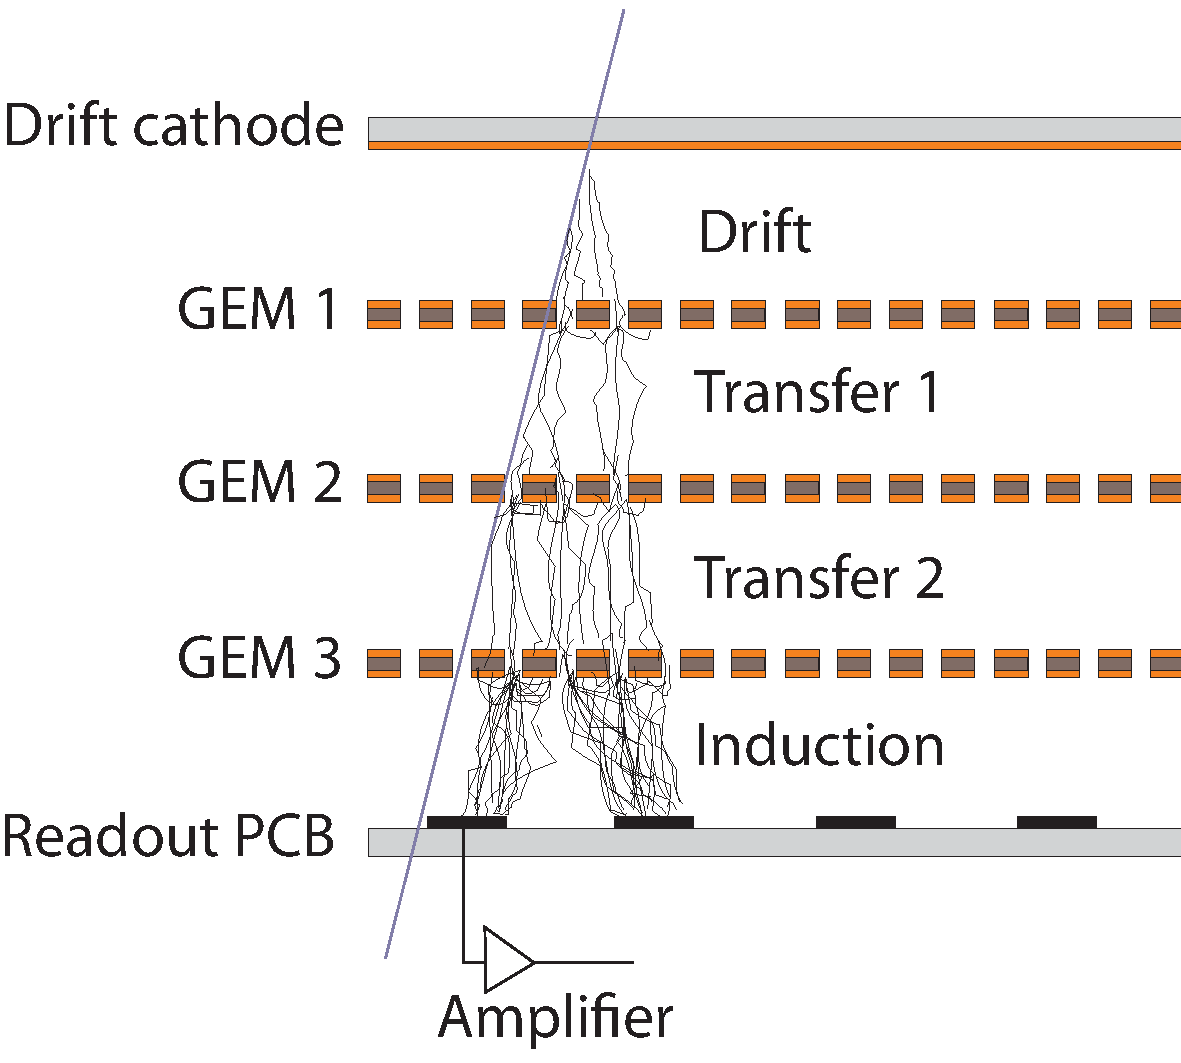
\includegraphics[width=0.5\textwidth]{img/II-1-gem/triple-gem-foils.pdf}
      \caption{??? \cite{Colaleo:2021453}.}
      \label{fig:II-1-gem-triple}
    \end{figure}

  \section{Technical Design of GE1/1 chambers for CMS}

      \begin{figure}[h!]
        \centering
        \includegraphics[width=\textwidth]{img/II-1-gem/gem-exploded.pdf}
        \caption{??? \cite{Colaleo:2021453}.}
        \label{fig:II-1-gem-exploded}
      \end{figure}

      \begin{figure}[h!]
        \centering
        \includegraphics[width=\textwidth]{img/II-1-gem/superchamber.pdf}
        \caption{??? \cite{Colaleo:2021453}.}
        \label{fig:II-1-gem-superchamber}
      \end{figure}

      \begin{figure}[h!]
        \centering
        \includegraphics[width=\textwidth]{img/II-1-gem/wheel.png}
        \caption{??? \cite{Colaleo:2021453}.}
        \label{fig:II-1-gem-wheel}
      \end{figure}

      \begin{figure}[h!]
        \centering
        \includegraphics[width=\textwidth]{img/II-1-gem/field-map.pdf}
        \caption{??? \cite{Colaleo:2021453}.}
        \label{fig:II-1-gem-field-map}
      \end{figure}

  \section{Detector Design Evolution}

    \begin{figure}[h!]
      \centering
      \includegraphics[width=\textwidth]{img/II-1-gem/generations.pdf}
      \caption{??? \cite{Colaleo:2021453}.}
      \label{fig:II-1-gem-generations}
    \end{figure}

  \section{GE1/1 Prototyping Results}

































  \section{GEM Upgrade Schedule}
